% Propósito: distinguir la suma instantánea de presiones coherentes de la suma
% de cuadrados eficaces para señales no correlacionadas.
% Origen: ecuaciones \eqref{eq:u4-suma-coherente} y
% \eqref{eq:u4-suma-no-correlacionada}, para dos señales de igual
% p_rms. Los incrementos son 20 log10(2)=6,02 dB y
% 10 log10(2)=3,01 dB.
% Esquema matemático; no representa mediciones ni fuentes particulares.
% Descripción accesible: el panel izquierdo muestra dos presiones coherentes
% iguales y en fase, que se suman hasta duplicar la presión y aumentar el nivel
% 6,02 dB. El derecho muestra dos presiones iguales no correlacionadas, cuyos
% cuadrados eficaces se suman; el RMS crece por raíz de dos y el nivel 3,01 dB.
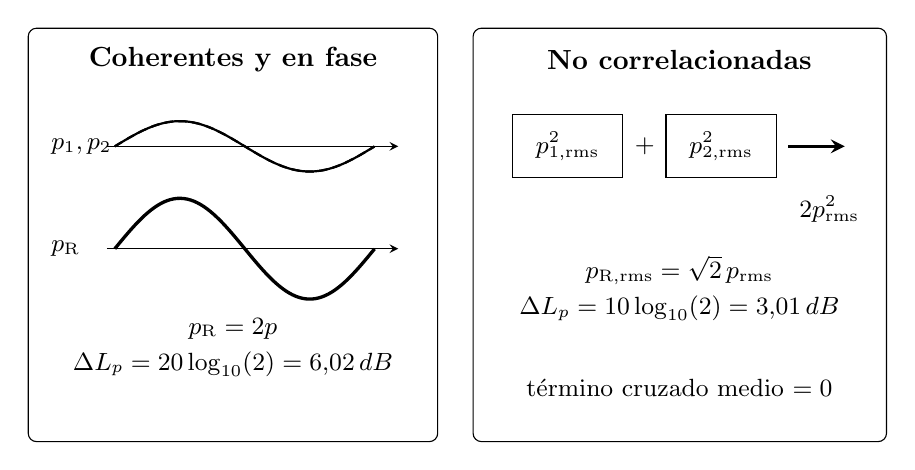
\begin{tikzpicture}[font=\small,>=stealth,x=1cm,y=1cm]
    \draw[rounded corners=3pt] (0.35,0.10) rectangle (5.55,5.35);
    \draw[rounded corners=3pt] (6.00,0.10) rectangle (11.25,5.35);

    \node[font=\bfseries] at (2.95,4.95) {Coherentes y en fase};
    \node[font=\bfseries] at (8.62,4.95) {No correlacionadas};

    \draw[->] (1.35,3.85) -- (5.05,3.85);
    \draw[thick,samples=80,domain=0:1]
        plot ({1.45+3.30*\x},{3.85+0.32*sin(360*\x)});
    \draw[thick,densely dashed,samples=80,domain=0:1]
        plot ({1.45+3.30*\x},{3.85+0.32*sin(360*\x)});
    \node[anchor=west] at (0.52,3.85) {\(p_1,p_2\)};

    \draw[->] (1.35,2.55) -- (5.05,2.55);
    \draw[very thick,samples=80,domain=0:1]
        plot ({1.45+3.30*\x},{2.55+0.64*sin(360*\x)});
    \node[anchor=west] at (0.52,2.55) {\(p_\mathrm{R}\)};

    \node[align=center] at (2.95,1.30)
        {\(p_\mathrm{R}=2p\)\\[2pt]
         \(\Delta L_p=20\log_{10}(2)=6{,}02\,\text{dB}\)};

    \node[draw,minimum width=1.40cm,minimum height=0.80cm] at (7.20,3.85)
        {\(p_{1,\mathrm{rms}}^2\)};
    \node at (8.18,3.85) {\(+\)};
    \node[draw,minimum width=1.40cm,minimum height=0.80cm] at (9.15,3.85)
        {\(p_{2,\mathrm{rms}}^2\)};
    \draw[->,very thick] (10.00,3.85) -- (10.72,3.85);
    \node[anchor=west,align=left] at (10.02,3.05)
        {\(2p_\mathrm{rms}^2\)};

    \node[align=center] at (8.62,2.05)
        {\(p_{\mathrm{R,rms}}=\sqrt{2}\,p_\mathrm{rms}\)\\[2pt]
         \(\Delta L_p=10\log_{10}(2)=3{,}01\,\text{dB}\)};
    \node[align=center] at (8.62,0.78)
        {término cruzado medio \(=0\)};
\end{tikzpicture}
